\chapter{จุลินทรีย์ในดินและวัฏจักรชีวธรณีเคมี}
\label{ch:soil_microbes}

\begin{keyconcept}[แนวคิดสำคัญของบทที่ 2]
ดินไม่ได้เป็นเพียงสสารทางกายภาพสำหรับการค้ำจุนต้นพืช แต่เป็นระบบนิเวศทางชีวภาพที่มีความหลากหลายสูงที่สุดแห่งหนึ่งบนโลก จุลินทรีย์ดิน (Soil Microorganisms)\index{จุลินทรีย์ดิน (Soil Microorganisms)} ทำหน้าที่เป็นโรงงานเคมีชีวภาพที่ขับเคลื่อนวัฏจักรชีวธรณีเคมี (Biogeochemical Cycles)\index{วัฏจักรชีวธรณีเคมี (Biogeochemical Cycles)} หลัก ได้แก่ วัฏจักรคาร์บอน ไนโตรเจน ฟอสฟอรัส และซัลเฟอร์ การเปลี่ยนรูปทางเคมีเหล่านี้กำหนดความพร้อมของธาตุอาหารที่พืชสามารถดูดซึมไปใช้ การสร้างอินทรียวัตถุในดิน และการกักเก็บคาร์บอนในระยะยาว (Soil Carbon Sequestration)\index{การกักเก็บคาร์บอนในดิน (Soil Carbon Sequestration)} ซึ่งเป็นหัวใจสำคัญของการฟื้นฟูความอุดมสมบูรณ์ของดินและการเกษตรที่ทนทานต่อสภาพภูมิอากาศ
\end{keyconcept}

\begin{figure}[ht]
    \centering
    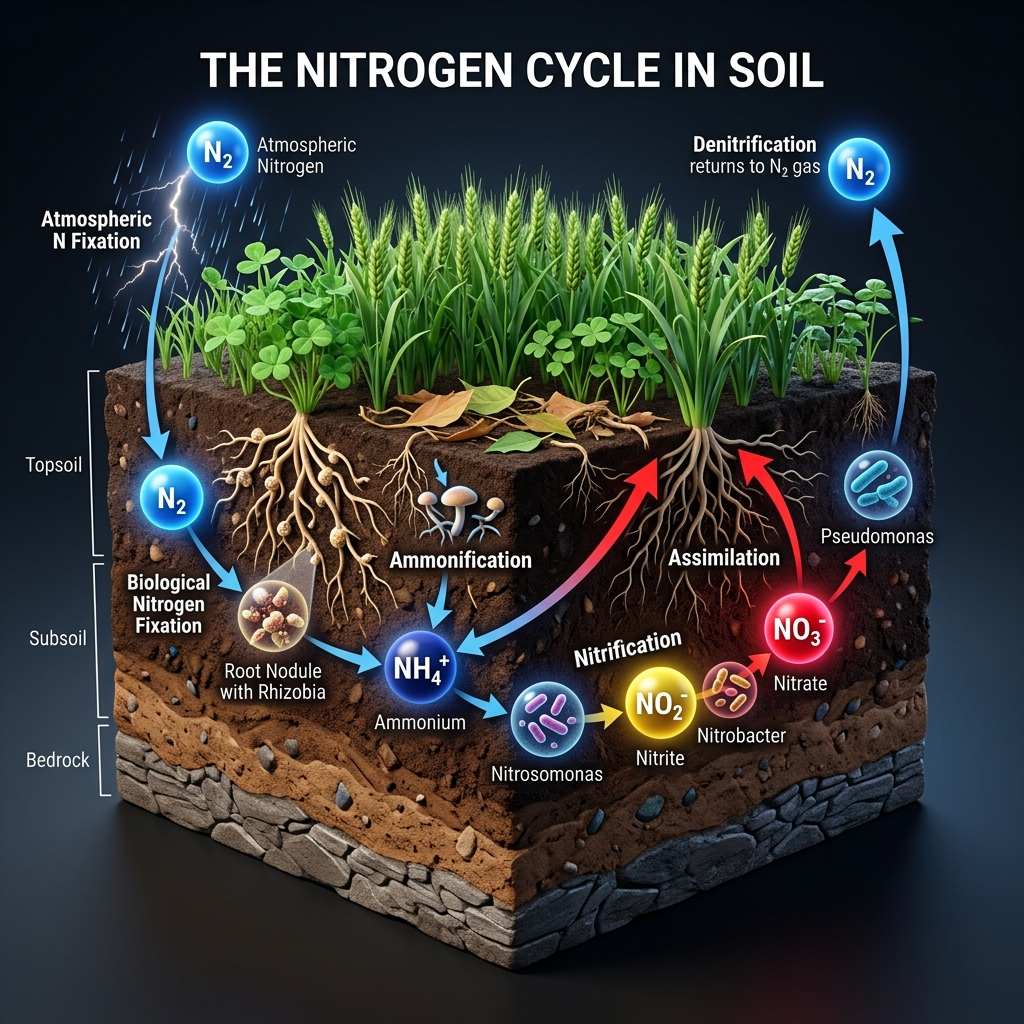
\includegraphics[width=0.85\textwidth]{assets/ch02_nitrogen_cycle.png}
    \caption{แผนภาพ 3D แสดงวัฏจักรไนโตรเจนในดินและเครือข่ายการทำงานร่วมกันของจุลินทรีย์ ตั้งแต่การตรึงไนโตรเจนทางชีวภาพ กระบวนการไนตริฟิเคชันโดยแบคทีเรียและอาร์เคีย ไปจนถึงกระบวนการดีไนตริฟิเคชันในสภาวะไร้ออกซิเจน}
    \label{fig:ch02_nitrogen_cycle}
\end{figure}

\section*{วัตถุประสงค์การเรียนรู้ประจำบท}
เมื่อศึกษาบทเรียนนี้จบแล้ว นักศึกษาสามารถ:
\begin{enumerate}
    \item จำแนกคุณลักษณะทางกายภาพ เคมี และชีวภาพของดินที่เป็นตัวกำหนดถิ่นที่อยู่อาศัยของจุลินทรีย์
    \item อธิบายกลไกการย่อยสลายสารอินทรีย์และทฤษฎีปั๊มคาร์บอนของจุลินทรีย์ (Microbial Carbon Pump) ในวัฏจักรคาร์บอน
    \item วิเคราะห์ขั้นตอนเคมีชีวภาพและสมการสมดุลในวัฏจักรไนโตรเจน (BNF, Nitrification, Denitrification, Anammox)
    \item อธิบายกลไกการละลายฟอสฟอรัสและวัฏจักรซัลเฟอร์ในดินกรดและดินน้ำขัง
    \item คำนวณสมดุลการตรึงไนโตรเจนและการเปลี่ยนแปลงอัตราส่วน C:N ต่อกระบวนการ Mineralization และ Immobilization
\end{enumerate}

\section{ดินในฐานะแหล่งที่อยู่อาศัยของจุลินทรีย์ (Soil as a Microbial Habitat)}

ดินเป็นระบบสามเฟสที่ประกอบด้วยเฟสของแข็ง (แร่ธาตุอนินทรีย์ 45\% และอินทรียวัตถุ 5\%) เฟสของเหลว (สารละลายดิน 25\%) และเฟสก๊าซ (อากาศในดิน 25\%) โครงสร้างเม็ดดิน (Soil Aggregates) ถูกจำแนกออกเป็นเม็ดดินขนาดใหญ่ (Macroaggregates, $>250\,\mu\text{m}$) และเม็ดดินขนาดเล็ก (Microaggregates, $<250\,\mu\text{m}$) 

ภายในเม็ดดินเหล่านี้มีช่องว่างระหว่างอนุภาค (Pore Network) ซึ่งสร้างไมโครแฮบิแทต (Microhabitats) ที่หลากหลาย จุลินทรีย์ดินส่วนใหญ่อาศัยอยู่รวมกันเป็นแผ่นฟิล์มชีวภาพ (Biofilms) เกาะติดกับผิวแร่ดินเหนียวและสารฮิวมัส โดยมีปัจจัยทางสิ่งแวดล้อมควบคุมกิจกรรมดังนี้:

\begin{itemize}
    \item \textbf{ความเป็นกรด-ด่างของดิน (Soil pH):} เป็นปัจจัยหลักที่กำหนดองค์ประกอบชุมชนจุลินทรีย์ ในดินกรด ($\text{pH} < 5.5$) เชื้อราจะมีความได้เปรียบในการเจริญเติบโตเนื่องจากทนกรดได้ดี ขณะที่แบคทีเรียส่วนใหญ่ชอบสภาวะเป็นกลางถึงด่างอ่อน ($\text{pH } 6.5$--$7.5$)
    \item \textbf{ศักย์รีดอกซ์ (Redox Potential, $E_h$):} บ่งชี้สถานะการถ่ายโอนอิเล็กตรอนในดิน ดินที่มีการถ่ายเทอากาศดีจะมีค่า $E_h > +400\text{ mV}$ (สภาวะใช้ออกซิเจน) ในขณะที่ดินน้ำขัง เช่น นาข้าว จะมีค่า $E_h$ ลดลงต่ำกว่า $-100\text{ mV}$ ทำให้เกิดสภาวะไม่ใช้ออกซิเจน
    \item \textbf{ศักย์ของน้ำในดิน (Soil Water Potential, $\psi$):} ควบคุมการเคลื่อนที่ของสารอาหารและการแพร่กระจายของแบคทีเรีย แบคทีเรียต้องการค่าน้ำอิสระสูง ($\psi > -0.5\text{ MPa}$) ในขณะที่เชื้อราสามารถทนต่อความแห้งแล้งได้สูงกว่ามาก ($\psi$ ต่ำถึง $-15\text{ MPa}$)
\end{itemize}

\section{วัฏจักรคาร์บอนและทฤษฎีปั๊มคาร์บอนของจุลินทรีย์ (Microbial Carbon Pump)}

คาร์บอนในดินมีปริมาณมากกว่าคาร์บอนในชั้นบรรยากาศและสิ่งมีชีวิตบนบกรวมกัน จุลินทรีย์ทำหน้าที่เป็นทั้งผู้ย่อยสลายและผู้กักเก็บคาร์บอน:

\subsection{การย่อยสลายสารอินทรีย์ลิกโนเซลลูโลส}

เศษซากพืชที่ตกลงสู่ดินประกอบด้วยพอลิเมอร์ที่ย่อยสลายยาก ได้แก่ เซลลูโลส (Cellulose, 40--50\%) เฮมิเซลลูโลส (Hemicellulose, 20--30\%) และลิกนิน (Lignin, 15--25\%) จุลินทรีย์หลั่งเอนไซม์ภายนอกเซลล์ (Extracellular Enzymes) มาย่อยสลาย:

\begin{itemize}
    \item \textbf{เอนไซม์เซลลูเลส (Cellulases):} ประกอบด้วย Endoglucanase, Exoglucanase (Cellobiohydrolase) และ $\beta$-Glucosidase ย่อยเซลลูโลสเป็นน้ำตาลกลูโคส
    \item \textbf{เอนไซม์ย่อยลิกนิน (Ligninases):} เชื้อรากลุ่ม White-rot fungi เช่น \organism{Phanerochaete chrysosporium} หลั่งเอนไซม์ Lignin Peroxidase (LiP), Manganese Peroxidase (MnP) และ Laccase ซึ่งใช้ปฏิกิริยาอนุมูลอิสระในการทำลายพันธะอีเทอร์และคาร์บอน-คาร์บอนในโครงสร้างลิกนิน
\end{itemize}

\subsection{แบบจำลอง Microbial Carbon Pump (MCP)}

แนวคิดดั้งเดิมเชื่อว่าฮิวมัสเกิดจากการสังเคราะห์สารประกอบฮิวมิกที่ไม่สามารถย่อยสลายได้ทางเคมี แต่หลักฐานทางวิทยาศาสตร์ยุคใหม่ค้นพบว่า \textbf{อินทรียวัตถุในดินส่วนใหญ่มีต้นกำเนิดมาจากซากเซลล์จุลินทรีย์ (Microbial Necromass)\index{ซากเซลล์จุลินทรีย์ (Microbial Necromass)}} ผ่านกลไกที่เรียกว่า \textbf{Microbial Carbon Pump (MCP)\index{Microbial Carbon Pump (MCP)}}:

\begin{equation}
\begin{split}
\text{Plant Residues} &\xrightarrow{\text{Anabolic Assimilation}} \text{Microbial Biomass} \\
&\xrightarrow{\text{Cell Turnover/Death}} \text{Necromass (Amino sugars, Lipids)} \\
&\xrightarrow{\text{Mineral Association}} \text{MAOM (Stabilized Carbon)}
\end{split}
\end{equation}

\begin{figure}[ht]
\centering
\begin{tikzpicture}[node distance=1.5cm, auto,
    proc/.style={rectangle, draw=agriGreen, fill=agriGrayBox, text width=3.3cm, rounded corners, minimum height=1.0cm, align=center, font=\small},
    storage/.style={rectangle, draw=agriBrown, fill=agriBrown!10, text width=3.3cm, rounded corners, minimum height=1.0cm, align=center, font=\small},
    arrow/.style={thick, ->, >=stealth, color=agriGreen}]
    
    \node [proc] (plant) {\textbf{เศษซากพืช (Plant Input)}\\สารคาร์บอนและสารคั้นราก};
    \node [proc, right=1.2cm of plant] (biomass) {\textbf{ชีวมวลจุลินทรีย์ (Biomass)}\\กระบวนการ In Vivo Assimilation};
    \node [proc, below=1.0cm of biomass] (necro) {\textbf{ซากเซลล์ (Necromass)}\\Amino sugars, Muramic acid};
    \node [storage, below=1.0cm of plant] (pom) {\textbf{Particulate Organic (POM)}\\กึ่งเสถียร (สลายตัวใน 1-10 ปี)};
    \node [storage, below=1.0cm of necro] (maom) {\textbf{Mineral-Associated (MAOM)}\\เกาะผิวแร่ดินเหนียว ($> 100$ ปี)};
    
    \draw [arrow] (plant) -- node[above]{\footnotesize ดูดซึมสร้างเซลล์} (biomass);
    \draw [arrow] (biomass) -- node[right]{\footnotesize การหมุนเวียนเซลล์ตาย} (necro);
    \draw [arrow] (necro) -- node[right]{\footnotesize พันธะออร์กาโนมิเนอรัล} (maom);
    \draw [arrow, dashed, color=agriBrown] (plant) -- node[left]{\footnotesize ย่อยสลายโครงสร้าง} (pom);
    \draw [arrow, dashed, color=agriBrown] (pom) -| node[pos=0.25, below]{\footnotesize ปลดปล่อย C ละลายน้ำ} (biomass);
\end{tikzpicture}
\caption{แผนผังกลไก Microbial Carbon Pump (MCP) แสดงเส้นทางหลักของการเปลี่ยนรูปสารอินทรีย์จากพืชสู่ซากจุลินทรีย์ (Microbial Necromass) และการจับยึดกับแร่ในดินเป็นคาร์บอนเสถียรภาพสูง MAOM}
\label{fig:mcp_diagram}
\end{figure}

ซากเซลล์จุลินทรีย์จะเข้าจับกับอนุภาคแร่ดินเหนียวกลายเป็น Mineral-Associated Organic Matter (MAOM)\index{MAOM (Mineral-Associated Organic Matter)} ซึ่งมีความคงทนสูงและกักเก็บคาร์บอนไว้ในดินได้นานหลายร้อยปี

\section{วัฏจักรไนโตรเจนและกระบวนการทางชีวเคมีของจุลินทรีย์}

ไนโตรเจนเป็นธาตุอาหารที่พืชต้องการมากที่สุด จุลินทรีย์ขับเคลื่อนการเปลี่ยนรูปทางเคมีผ่าน 4 กระบวนการหลัก:

\subsection{1. การตรึงไนโตรเจนทางชีวภาพ (Biological Nitrogen Fixation: BNF)}

ปฏิกิริยาการเปลี่ยนก๊าซไนโตรเจน ($N_2$) จากอากาศเป็นแอมโมเนีย ($NH_3$) อาศัยเอนไซม์ไนโตรจีเนส (Nitrogenase Complex)\index{การตรึงไนโตรเจนทางชีวภาพ (BNF)}\index{เอนไซม์ไนโตรจีเนส (Nitrogenase Complex)} ซึ่งประกอบด้วยโปรตีน 2 ชนิด:
\begin{enumerate}
    \item \textbf{Dinitrogenase Reductase (Fe protein):} ทำหน้าที่รับอิเล็กตรอนจากเฟอร์รีดอกซิน (Ferredoxin) และจับกับ ATP
    \item \textbf{Dinitrogenase (MoFe protein):} มีศูนย์กลางเร่งปฏิกิริยา FeMo-cofactor ทำหน้าที่ส่งผ่านอิเล็กตรอนไปรีดิวซ์ $N_2$
\end{enumerate}

\begin{equation}
N_2 + 8H^+ + 8e^- + 16\text{ATP} \xrightarrow{\text{nitrogenase}} 2NH_3 + H_2 + 16\text{ADP} + 16\text{P}_i
\label{eq:bnf_full}
\end{equation}

เอนไซม์ไนโตรจีเนสจะสูญเสียการทำงานทันทีเมื่อสัมผัสกับออกซิเจน จุลินทรีย์จึงพัฒนากลไกป้องกันออกซิเจน เช่น โปรตีนเลกเฮโมโกลบิน (Leghemoglobin)\index{เลกเฮโมโกลบิน (Leghemoglobin)} ในปมรากถั่ว, เซลล์เฮเทอโรซีสต์ (Heterocyst)\index{เฮเทอโรซีสต์ (Heterocyst)} ในไซยาโนแบคทีเรีย, และอัตราการหายใจระดับเซลล์ที่สูงมากใน \organism{Azotobacter}

\subsection{2. กระบวนการไนตริฟิเคชัน (Nitrification)}

การออกซิไดซ์แอมโมเนียเป็นไนเตรตแบ่งออกเป็น 2 ขั้นตอน:\index{ไนตริฟิเคชัน (Nitrification)}

\textbf{ขั้นที่ 1: การเปลี่ยนแอมโมเนียมเป็นไนไตรต์} ขับเคลื่อนโดยแบคทีเรียออกซิไดซ์แอมโมเนีย (Ammonia-Oxidizing Bacteria: AOB\index{แบคทีเรียออกซิไดซ์แอมโมเนีย (AOB)} เช่น \organism{Nitrosomonas}\index{Nitrosomonas@\textit{Nitrosomonas}}) และอาร์เคียออกซิไดซ์แอมโมเนีย (Ammonia-Oxidizing Archaea: AOA เช่น \organism{Nitrososphaera}) ซึ่งมีเอนไซม์ Ammonia Monooxygenase (AMO):
\begin{equation}
2NH_4^+ + 3O_2 \rightarrow 2NO_2^- + 4H^+ + 2H_2O \quad (\Delta G^\circ = -544\text{ kJ})
\end{equation}

\textbf{ขั้นที่ 2: การเปลี่ยนไนไตรต์เป็นไนเตรต} ขับเคลื่อนโดย Nitrite-Oxidizing Bacteria (NOB\index{แบคทีเรียออกซิไดซ์ไนไตรต์ (NOB)} เช่น \organism{Nitrobacter}\index{Nitrobacter@\textit{Nitrobacter}}, \organism{Nitrospira}) ผ่านเอนไซม์ Nitrite Oxidoreductase (NXR):
\begin{equation}
2NO_2^- + O_2 \rightarrow 2NO_3^- \quad (\Delta G^\circ = -153\text{ kJ})
\end{equation}

\subsection{3. กระบวนการดีไนตริฟิเคชัน (Denitrification)}

ในสภาวะขาดออกซิเจน แบคทีเรียกลุ่มไม่ใช้ออกซิเจนแบบเผื่อเลือก (เช่น \organism{Pseudomonas}, \organism{Paracoccus}) จะใช้สารประกอบไนโตรเจนออกไซด์เป็นตัวรับอิเล็กตรอนสุดท้ายในห่วงโซ่การหายใจ:\index{ดีไนตริฟิเคชัน (Denitrification)}

\begin{equation}
NO_3^- \xrightarrow{\text{Nar}} NO_2^- \xrightarrow{\text{Nir}} NO \xrightarrow{\text{Nor}} N_2O \xrightarrow{\text{Nos}} N_2
\end{equation}

หากเอนไซม์ Nitrous Oxide Reductase (Nos) ถูกยับยั้งจากความเป็นกรดในดิน จะส่งผลให้ก๊าซไนตรัสออกไซด์ ($N_2O$)\index{ก๊าซไนตรัสออกไซด์ ($N_2O$)} ซึ่งเป็นก๊าซเรือนกระจกที่มีศักยภาพทำให้โลกร้อนสูงกว่า $CO_2$ ถึง 298 เท่า ถูกปลดปล่อยสู่บรรยากาศ

\section{วัฏจักรฟอสฟอรัสและซัลเฟอร์ในดิน}

\subsection{การละลายฟอสเฟตโดยจุลินทรีย์ (Phosphate Solubilization)}

ฟอสฟอรัสในดินร้อยละ 95--99 อยู่ในรูปที่ไม่ละลายน้ำ โดยในดินกรดจะตกตะกอนร่วมกับเหล็กและอะลูมิเนียม ($FePO_4, AlPO_4$) ส่วนในดินด่างจะตกตะกอนร่วมกับแคลเซียม ($Ca_3(PO_4)_2$) จุลินทรีย์กลุ่ม Phosphate-Solubilizing Microorganisms (PSM)\index{แบคทีเรียละลายฟอสเฟต (PSB)}\index{การละลายฟอสเฟต (Phosphate Solubilization)} เช่น \organism{Bacillus megaterium}, \organism{Pseudomonas putida}, และ \organism{Aspergillus niger} ปลดปล่อยฟอสเฟตผ่าน 2 กลไก:

\begin{enumerate}
    \item \textbf{การหลั่งกรดอินทรีย์โมเลกุลต่ำ (Low Molecular Weight Organic Acids):} เช่น กรดกลูโคนิก (Gluconic acid)\index{กรดกลูโคนิก (Gluconic acid)} กรดซิตริก (Citric acid) และกรดออกซาลิก (Oxalic acid) กรดเหล่านี้ช่วยลดค่า pH และทำหน้าที่เป็นสารคีเลต (Chelating agents) แย่งจับประจุ $Ca^{2+}, Fe^{3+}, Al^{3+}$ ปลดปล่อยฟอสเฟตอิสระ ($H_2PO_4^-$)
    \item \textbf{การผลิตเอนไซม์ฟอสฟาเตสและไฟเตส (Phosphatases and Phytases):}\index{เอนไซม์ไฟเตส (Phytase)}\index{เอนไซม์ฟอสฟาเตส (Phosphatase)} ย่อยสลายสารประกอบฟอสฟอรัสอินทรีย์ เช่น กรดไฟติก (Phytic acid)\index{กรดไฟติก (Phytic acid)} ในดิน
\end{enumerate}

\subsection{วัฏจักรซัลเฟอร์และการเกิดดินเปรี้ยวจัด}

ในพื้นที่ลุ่มน้ำขังชายฝั่งทะเล เช่น แถบภาคกลางและภาคตะวันออก แบคทีเรียรีดิวซ์ซัลเฟต (\organism{Desulfovibrio}) จะเปลี่ยนซัลเฟตเป็นไฮโดรเจนซัลไฟด์และตกตะกอนร่วมกับเหล็กกลายเป็นแร่ไพไรต์ ($FeS_2$) เมื่อมีการขุดเปิดหน้าดินสัมผัสอากาศ แบคทีเรีย \organism{Acidithiobacillus ferrooxidans}\index{Acidithiobacillus ferrooxidans@\textit{Acidithiobacillus ferrooxidans}} จะเร่งปฏิกิริยาออกซิเดชันอย่างรวดเร็ว:

\begin{equation}
4FeS_2 + 15O_2 + 14H_2O \xrightarrow{\text{Acidithiobacillus}} 4Fe(OH)_3 + 8H_2SO_4
\end{equation}

กรดซัลฟิวริกที่เกิดขึ้นทำให้ดินมีค่า pH ลดลงต่ำกว่า 3.5 เกิดเป็น "ดินเปรี้ยวจัด (Acid Sulfate Soils)"\index{ดินเปรี้ยวจัด (Acid Sulfate Soils)} ซึ่งปลดปล่อยอะลูมิเนียมไอออนที่เป็นพิษร้ายแรงต่อรากพืช

\begin{worked}[ตัวอย่างที่ 2.1 การคำนวณสมดุลการตรึงไนโตรเจนและการทดแทนปุ๋ยยูเรีย]
แปลงปลูกถั่วเหลืองในพื้นที่จังหวัดจันทบุรีขนาด 5 ไร่ (ประมาณ 0.8 เฮกตาร์) มีการคลุกเมล็ดด้วยหัวเชื้อ \organism{Bradyrhizobium japonicum} อย่างมีประสิทธิภาพ สามารถตรึงไนโตรเจนได้เฉลี่ย $150\text{ kg N/ha/ปี}$
\begin{enumerate}
    \item จงคำนวณปริมาณไนโตรเจนบริสุทธิ์ที่ตรึงได้ทั้งหมดในแปลงนี้ต่อปี
    \item หากปุ๋ยเคมียูเรีย ($46\text{-}0\text{-}0$) มีปริมาณไนโตรเจน 46\% โดยน้ำหนัก แปลงนี้สามารถลดการใช้ปุ๋ยยูเรียได้กี่กิโลกรัมต่อปี?
\end{enumerate}

\textbf{วิธีทำ:}
1. ปริมาณไนโตรเจนที่ตรึงได้ในพื้นที่ 0.8 เฮกตาร์:
$$\text{Total N fixed} = 150\text{ kg N/ha} \times 0.8\text{ ha} = 120\text{ kg N/ปี}$$
2. การคำนวณเทียบเท่าน้ำหนักปุ๋ยยูเรีย (มี N 46\%):
$$\text{Weight of Urea} = \frac{120\text{ kg N}}{0.46} \approx 260.87\text{ kg ยูเรีย/ปี}$$
คิดเป็นกระสอบปุ๋ยยูเรีย (ขนาด 50 kg) ประมาณ $5.2$ กระสอบต่อปี ช่วยประหยัดต้นทุนและลดการชะล้างปุ๋ยลงแหล่งน้ำใต้ดิน
\end{worked}

\begin{worked}[ตัวอย่างที่ 2.2 การคำนวณอัตราส่วน C:N และการทำนายกระบวนการ Mineralization vs Immobilization]
เกษตรกรใส่เศษเหลือพืช 2 ชนิดลงในดิน:
\begin{itemize}
    \item แปลง ก: ใส่ฟางข้าวแห้งที่มีปริมาณคาร์บอน 40\% และไนโตรเจน 0.5\%
    \item แปลง ข: ใส่เศษซากถั่วเหลืองที่มีปริมาณคาร์บอน 42\% และไนโตรเจน 3.5\%
\end{itemize}
จงคำนวณอัตราส่วน C:N ของวัสดุทั้งสอง และทำนายว่าจะเกิดกระบวนการตรึงไนโตรเจนในเซลล์จุลินทรีย์ (Immobilization) หรือการปลดปล่อยไนโตรเจนให้พืช (Mineralization)?

\textbf{วิธีทำ:}
1. อัตราส่วน C:N แปลง ก (ฟางข้าว):
$$\text{C:N} = \frac{40\%}{0.5\%} = 80:1$$
2. อัตราส่วน C:N แปลง ข (เศษถั่ว):
$$\text{C:N} = \frac{42\%}{3.5\%} = 12:1$$

\textbf{บทวิเคราะห์ผลลัพธ์:}
\begin{itemize}
    \item เกณฑ์ตัดสินทางจุลชีววิทยาดิน: หากวัสดุมี $\text{C:N} > 25:1$--$30:1$ จุลินทรีย์จะมีไนโตรเจนไม่เพียงพอต่อการสร้างโปรตีนในเซลล์ จึงต้องแย่งชิงไนโตรเจนอิสระในดินมาใช้ เกิดภาวะ **Immobilization (การตรึงชั่วคราว)** ส่งผลให้พืชเกิดอาการขาดไนโตรเจนใบเหลืองชั่วคราวในแปลง ก
    \item ในแปลง ข มี $\text{C:N} = 12:1$ ซึ่งต่ำกว่า $20:1$ จุลินทรีย์มีไนโตรเจนเกินความต้องการ จึงปลดปล่อยแอมโมเนียมส่วนเกินออกสู่ดินผ่านกระบวนการ **Net Mineralization** ทำให้พืชได้รับไนโตรเจนไปใช้ในการเจริญเติบโตทันที
\end{itemize}
\end{worked}

% [RESEARCH-UPDATE-2026-10]
\section{ความก้าวหน้างานวิจัยล่าสุดด้านจุลินทรีย์ดินและคาร์บอน}

การศึกษาเชิงลึกระดับโลกในปี ค.ศ. 2024 โดย Hu และคณะ \cite{pmid39172788} ในวารสาร *PNAS* ได้พัฒนาระบบประเมินปริมาณการกักเก็บคาร์บอนจากซากจุลินทรีย์ดิน โดยชี้ว่าสัดส่วนของ Necromass-derived carbon มีสัดส่วนมากกว่าร้อยละ 50 ของคาร์บอนอินทรีย์ทั้งหมดในดินชั้นบน 

สอดคล้องกับงานวิจัยของ Cui และคณะ \cite{pmid39024521} ในวารสาร *Advanced Science* ที่ค้นพบว่าประสิทธิภาพการใช้คาร์บอนของจุลินทรีย์ (Microbial Carbon Use Efficiency: CUE) ถูกจำกัดด้วยสัดส่วนธาตุอาหารฟอสฟอรัสในดินเขตร้อนมากกว่าไนโตรเจน การปรับสมดุลชีวธรณีเคมีด้วยปุ๋ยชีวภาพจึงมีผลโดยตรงต่อการบรรเทาภาวะโลกร้อน

\begin{insight}[ประเด็นวิเคราะห์เชิงวิชาการ]
เกษตรกรที่ปลูกไม้ผลมักใส่ปุ๋ยอินทรีย์ร่วมกับปุ๋ยเคมี จากหลักการ Microbial Carbon Use Efficiency (CUE) เราควรออกแบบตารางการให้สารอาหารแก่ดินอย่างไรเพื่อเพิ่มทั้งการดูดซึมของรากพืชและการสร้างคาร์บอนสะสมในดินระยะยาว?
\end{insight}

\section*{สรุปประจำบท}

ดินเป็นถิ่นที่อยู่อาศัยอันอุดมสมบูรณ์ของจุลินทรีย์ที่ทำหน้าที่เป็นกลไกหลักในวัฏจักรชีวธรณีเคมี การย่อยสลายสารอินทรีย์ไม่ได้ยุติลงที่การสลายตัวของเศษพืช แต่ถูกแปรรูปผ่านกระบวนการอะนาบอลิซึมของจุลินทรีย์กลายเป็น Microbial Necromass ที่สร้างความยั่งยืนของคาร์บอนในดิน วัฏจักรไนโตรเจน ฟอสฟอรัส และซัลเฟอร์ ดำเนินไปอย่างสมดุลผ่านการประสานงานของกลุ่มจุลินทรีย์ที่มีความจำเพาะทางเอนไซม์ การบริหารจัดการอัตราส่วน C:N และการรักษาสมดุลรีดอกซ์จึงเป็นกุญแจสำคัญในการยกระดับผลผลิตพืชและการอนุรักษ์ดิน

\subsection*{คำถามท้ายบทและการวิเคราะห์}

\noindent \textbf{ระดับที่ 1: ความรู้และความเข้าใจเชิงทฤษฎี (Knowledge \& Comprehension)}
\begin{enumerate}
    \item อธิบายลักษณะโครงสร้างของเม็ดดิน (Micro- และ Macroaggregates) และวิเคราะห์ว่าช่องว่างระหว่างอนุภาคส่งผลต่อความหลากหลายของจุลินทรีย์อย่างไร
    \item เปรียบเทียบความแตกต่างระหว่างแนวคิดดั้งเดิมเรื่องการเกิดฮิวมัส (Humification) กับทฤษฎีปั๊มคาร์บอนของจุลินทรีย์ (Microbial Carbon Pump: MCP)
    \item เอนไซม์ไนโตรจีเนสประกอบด้วยโปรตีนกี่ส่วน แต่ละส่วนทำหน้าที่อย่างไร และเพราะเหตุใดจึงจำเป็นต้องใช้พลังงาน ATP สูงถึง 16 โมเลกุลต่อ 1 โมเลกุลของ $N_2$?
    \item วิเคราะห์บทบาทของแบคทีเรียกลุ่ม AOB และ NOB ในกระบวนการไนตริฟิเคชัน และอธิบายผลกระทบของกระบวนการนี้ต่อค่าความเป็นกรด-ด่างของดิน
\end{enumerate}

\noindent \textbf{ระดับที่ 2: การวิเคราะห์และการคำนวณเชิงปริมาณ (Quantitative Analysis \& Calculation)}
\begin{enumerate}[resume]
    \item ปัจจัยใดในดินที่กระตุ้นให้เกิดการปลดปล่อยก๊าซไนตรัสออกไซด์ ($N_2O$) ในกระบวนการดีไนตริฟิเคชัน และเกษตรกรสามารถควบคุมได้อย่างไร?
    \item อธิบายกลไกการละลายฟอสฟอรัสที่ตกตะกอนร่วมกับไอออนแคลเซียม ($Ca^{2+}$) และไอออนเหล็ก ($Fe^{3+}$) ของจุลินทรีย์กลุ่ม PSM
    \item หากแปลงเกษตรมีเศษฟางข้าวสับ 2,000 กิโลกรัม ($\text{C:N} = 80:1$, คาร์บอน 40\%) เกษตรกรควรเติมมูลไก่สด ($\text{C:N} = 10:1$, คาร์บอน 30\%) ปริมาณกี่กิโลกรัม เพื่อปรับให้อัตราส่วน C:N รวมมีค่าเท่ากับ $25:1$?
\end{enumerate}

\noindent \textbf{ระดับที่ 3: การสังเคราะห์และการแก้ปัญหาในแปลงจริง (Application \& Real-World Synthesis)}
\begin{enumerate}[resume]
    \item ในการเกิดดินเปรี้ยวจัด แบคทีเรีย \organism{Acidithiobacillus ferrooxidans} มีบทบาททางชีวเคมีอย่างไรในการเร่งปฏิกิริยาการเกิดกรดซัลฟิวริก และควรมีแนวทางฟื้นฟูดินอย่างไร?
    \item อธิบายกระบวนการแอนาม็อกซ์ (Anammox) และความแตกต่างเมื่อเปรียบเทียบกับกระบวนการดีไนตริฟิเคชันแบบดั้งเดิมในดินน้ำขัง
    \item จากงานวิจัยของ Cui และคณะ (2024) เหตุใดประสิทธิภาพการใช้คาร์บอนของจุลินทรีย์ (CUE) ในดินเขตร้อนจึงขึ้นอยู่กับความพร้อมของฟอสฟอรัส และจะนำมาใช้วางแผนการให้ปุ๋ยชีวภาพในสวนผลไม้อย่างไร?
\end{enumerate}
